\documentclass[a4paper]{article}
\usepackage{graphicx}
\usepackage{a4wide}
\usepackage{moreverb}
\usepackage{multicol}

\title{\Large{ \textsc{ 640-364 Computational Physics --- Project 5} } \\[3mm]
       \bfseries{{\huge Gravitational Lensing by Point Masses}}}
\author{Michael Papasimeon}
\date{October 29, 1997}

\begin{document}
\maketitle

\section{Aims}
The general aim is to investigate the effect of gravitational lensing through the 
use of computer simulation. The specific aims are to:
\begin{itemize}
    \item Investigate the effects of distance on gravitational lensing
          by solving the Dyer-Roeder equation for different cosmologies.
    \item Write a computer program which lenses an extended source image 
          represented as a 2D grid. 
    \item Investigate the critical and caustic curves for a number of different
          situations.
\end{itemize}

\section{Theory}
%\begin{multicols}{2}
According to Einstein's General Theory of Relativity, the path a light
ray travels is deflected when it passes close to an object with a large
enough gravitational field. The amount of angular deflection depends on
the mass of the deflecting object, and the distance between the light and
the object. The effect is known as gravitational lensing as the deflecting
object acts very much like an optical lens, in that images of distant
stellar objects can be magnified, distorted, focused and multiple
images being created.
\begin{center}
        \includegraphics[width=7cm]{images/hubble.eps}
        \\[1mm]
        Figure 1: Gravitational Lens in Abbell 2218
\end{center}

The effect has been observed many times using both ground and spaced
based telesopes at both optical and radio wavelengths. The lensing objects
are usually galaxies, but may also be other objects with large masses
such as neutron stars and black holes. 

Gravitational lensing has many applications in astronomy and astrophysics
as the deflection angle of the light allows to calculate the mass
of the deflecting object accurately. This technique allows the mass determination
of non-lumnous astrophysical objects such as black holes.
The main problem with observing gravitational lenses is that close
alignment is needed between the Earth, the deflecting object and 
the source object to observe the effect. Therefore, many of the gravitational
lenses observed involve distant galaxies and quasars as the source objects.

Figure 1 shows an example of a gravitational lens taken with the 
Hubble Space Telescope. The bright galaxy in the centre right of the image
has graviationally lensed a galaxy which is located behind it. 
The large arcs around the deflecting galaxy are multiple images of 
a distant source galaxy.

\subsection{The Lens Equation}
Shown in figure 2, the angular deflection $\alpha$ of a 
gravitational lense is given by
\begin{equation}    
    \alpha = \frac{4GM}{c^2 \xi}
\end{equation}
where
\begin{itemize}
    \item $M = $ mass of the deflecting object
    \item $G = $ gravitational constant
    \item $c = $ speed of light
    \item $\xi = $ impact radius of the incoming photon
    \item $\alpha = $ deflection angle
\end{itemize}
\begin{center}
    \includegraphics[width=7cm]{images/gldiag.eps}
    \\[1mm]
    Figure 2 : Angular Deflection of a Photon
\end{center}

The deflecting mass may be viewed as an optical thin lens, made up
of a two dimensional mass distribution.
\begin{equation}
    M = \int_{R^2} \Sigma(\vec{\xi '}) 
        \frac{\vec{\xi} - \vec{\xi '} }{|\vec{\xi} - \vec{\xi '}|^2} d^2 \xi '
\end{equation}
where
\begin{itemize}
    \item $\Sigma = $ surface density
    \item $R^2 = $ surface area
\end{itemize}
If the deflecting mass, is perfectly symmetric, the deflection angle becomes
\begin{equation}
    \vec{\alpha} = \frac{4GM(<\xi)\vec{\xi}}{c^2|\vec{\xi}|^2}
\end{equation}

Figure 3 below shows the setup for the lens equation. The lens
equation is
\begin{equation}
    \psi D_{os} + \alpha D_{ds} = \beta D_{os}
\end{equation}
It is often the case in many gravitational lensing problems that 
the images form do not depend on the distances between source, observer
and deflector directly. Rather a specific ratio of these distances
is the quantity which needs to be considered. This is known as the
effective distance $D$ and is defined as:
\begin{equation}
\label{eq:effd}
    D = \frac{D_{od} D_{ds} }{D_{os}}
\end{equation}
\begin{center}
    \includegraphics[angle=-90,width=7cm]{images/setup.eps}
    \\[1mm]
    Figure 3: Setup for the lens equation
\end{center}

\subsection{Point Mass Lenses}
Certain gravitational lenses may be approximated as point masses. 
These include large mass objects such as black holes and neutron stars.
If a distant star is in perfect alignment with a point mass gravitational
lens and an observer, the light from the distant star is lensed 
perfectly symmetrically forming a ring image of the star known as an
Einstein ring. The radius of the Einstein ring is given by
\begin{equation}
    \theta_{E} = \sqrt{\frac{4GM}{c^2} \frac{D_{ds}}{D_{od} D_{os}}}
\end{equation}
If however there isn't a perfect alignment, for a point mass two
images are produced for each point on the source plane. 
The angular positions at which these images is given by:
\begin{equation}
    \theta_{\pm} = \frac{\xi}{D_{od}}
                 = \frac{\beta}{2} \pm \sqrt{\beta^2 + 4\theta^{2}_{E}}
\end{equation}
where $\beta$ is the angular position of the source as shown in figure 3.
The magnification of each of the images is given by
\begin{equation}
    \mu_{\pm} = \frac{1}{4} 
                \left[ 
                    \frac{y}{\sqrt{y^2 + 4}} 
                    +
                    \frac{\sqrt{y^2 + 4}}{y} 
                    \pm 2
                \right]
\end{equation}
where the source and image angles have been scaled such that 
$y = \psi / \alpha_0$ and $x = \alpha / \alpha_0$.

Using this notation the lens equation can be rewritten as the scaled
lens equation given by
\begin{equation}
    \vec{y} = \vec{x} - \vec{\alpha}(\vec{x}).
\end{equation}
The vector notation used represents the coordinate in a cartesian plane.
Therefore
\begin{itemize}
    \item $\vec{y} = (y_1, y_2)$ is a coordinate in the source plane and
    \item $\vec{x} = (x_1, x_2)$ is a coordinate in the deflecting plane.
\end{itemize}
This can also be written using complex number notation. A position in 
deflecting plane can be denoted as $z = x_1 + ix_2$, and a position in the
source plane as $z_s = y_1 + iy_2$.

The magnification is given by:
\begin{equation}
    \mu(\vec{x}) = \frac{1}{det A(\vec{x})}
\end{equation}
where $det A(\vec{x})$ is the Jacobian determinant of the Hessian matrix
given by
\begin{equation}
    A(\vec{x}) = \frac{\partial \vec{y}}{\partial \vec{x}}
\end{equation}

\subsection{Critical Curves and Caustics}
Critical curves are the set of all points in the deflection plane where
$A(\vec{x}) = 0$. The corresponding curves in the source plane (obtained
from the lens equation) are known as caustics. Critical curves are where
the gravitational lens infinitely magnifies the light passing through
that point. Source plane caustics are the pre-image of the critical curves.
Any light emitted near a caustic will be greatly magnified as it passes
through the lens. 

\subsection{The Chang-Refsdal Lens}
The Chang-Refsdal lens model describes gravitational lensing using a modification
of the point mass model. This model says that when a source crosses a fold caustic
the lensing is due to a point mass but with an additional external shear applied.
The corresponding lens equation for the Chang-Refsdal model is:
\begin{equation}
    \vec{y} = \left[
                \begin{array}{cc}
                    1 + \gamma & 0   \\
                    0          & 1 - \gamma
                \end{array} 
              \right] \vec{x} - \frac{\vec{x}}{|\vec{x}|^2}
\end{equation}
This can also be written in the complex notation as 
$z_s = z + \gamma \bar{z} - \frac{\epsilon}{\bar{z}}$, where
\begin{itemize}
    \item $\gamma$ is a constant determining the amount shear.
    \item $\epsilon = (\frac{\kappa_s}{1 - \kappa_c})$, where $\kappa_s$ is
          the density of compact objects such as stars and $\kappa_c$ is the
          surface density of continuously distributed matter.
\end{itemize}

%\end{multicols}

\section{The Effects of Distance on Gravitational Lensing}
\subsection{Method} 
The Dyer-Roeder equation is given by:
\begin{equation}
    (z+1)(\Omega z + 1) \frac{d^2D}{dz^2} + 
    \left( \frac{7}{2}\Omega z + \frac{1}{2}\Omega + 3 \right) \frac{dD}{dz} + 
    \frac{3}{2} \tilde{\alpha} \Omega D = 0
\end{equation}
This relates the angular diameter distance of a lensing system with the
redshift $z$ of the source object.
\begin{itemize}
    \item $\Omega$ is the ratio of the mean mass density to the critical
          density of the universe and
    \item $\tilde{\alpha}$ is the clumpiness parameter, which determines
          the amount of matter between the source and the observer.
\end{itemize}
The initial conditions of the Dyer-Roeder equation are:
\begin{equation}
    D_{ii} = 0
\end{equation}
\begin{equation}
    \left[ \frac{dD_{ij}}{dz} \right]_{z_j = z_i} =
         \frac{\mathrm{sgn} (z_j - z_i)}{(z_i + 1)^2 \sqrt{\Omega z_i + 1} }
\end{equation}

The Dyer-Roeder equation needs to be solved for three different cases.
\begin{enumerate}
    \item  $\Omega = 0$ $(D_{I})$
    \item  $\Omega = 1$, $\tilde{\alpha} = 1$ $(D_{II})$
    \item  $\Omega = 1$, $\tilde{\alpha} = 0$ $(D_{III})$
\end{enumerate}

This leads to three different equations which need to be solved.
\begin{equation}
    (z+1)\frac{d^2D}{dz^2} + 3 \frac{dD}{dz} = 0
\end{equation}

\begin{equation}
    (z+1)^2 \frac{d^2D}{dz^2} + \frac{7}{2}(z+1)\frac{dD}{dz} + \frac{3}{2}D = 0
\end{equation}

\begin{equation}
    (z+1)^2 \frac{d^2D}{dz^2} + \frac{7}{2}(z+1)\frac{dD}{dz} = 0
\end{equation}

A FORTRAN program (see Appendix B -- \texttt{lense.f}) was written
to numerically solve these equations. The algorithm used to solve these
equation numerically was the \emph{Runge-Kutta-Nystr\"{o}m}~\footnote{
See the code in Appendix B for the exact algorithm. This algorithm
was obtained from Chapter 20 (Numerical Methods for Differential Equations)
from \emph{Advanced Engineering Mathematics} by Erwin Kreyszig.}
method.  Is method is a fourth order algorithm which is a general form 
of the standard \emph{Runge-Kutta} method, used for solving second order 
ordinary differential equations.

The equations were integrated from $z = 0$ to $z = 10$. 
Also, the dimming factor $(D_{II}/D_{III})^2$ was determined and plotted
as a function of redshift $z$.

\subsection{Results and Discussion} 
The plot below shows the numerical result of solving the Dyer-Roeder
equation for the three different cosmologies resulting in three
solutions for the angular diameter distance $D$.
\begin{itemize}
    \item $D_{I}$   \texttt{d1.dat} (The top curve)
    \item $D_{II}$  \texttt{d2.dat} (The bottom curve)
    \item $D_{III}$ \texttt{d3.dat} (The centre curve)
\end{itemize}
\begin{center}
    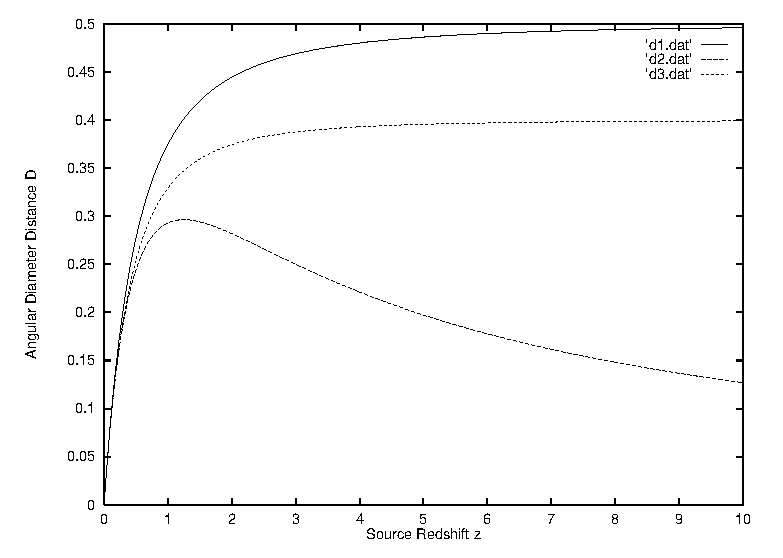
\includegraphics{Results/cosmo_all.eps}
    \\[1mm]
    Plot of Angular Diameter Distance against Source Redshift
\end{center}
According to the big bang model of the universe, objects with large
redshifts are further away. Hence the results of solving the Dyer-Roeder
equation for the cases (1 and 3) when the ``clumpiness'' parameter 
$\tilde{\alpha}$ is ignored the angular diameter distance $D$ increases
as the redshift increases. In both cases we get asymptoting values:
\begin{equation}
    \lim_{z \rightarrow \infty} D_{I}(z) = 0.5
\end{equation}
\begin{equation}
    \lim_{z \rightarrow \infty} D_{II}(z) = 0.4
\end{equation}
In both these cases where $\tilde{\alpha}$ is not in the equation, 
the lens is the only matter along the line of sight to the source and
hence we get an increase in the angular diameter distance as the redshift 
increases. Of particular interest is that in case $I$ ($\Omega = 0$), 
the value of $D$ increases more rapidly than in case $III$ ($\Omega = 1$).
Hence we see that the density of the universe plays influences the results
of any models chosen for gravitational lensing. Since the mean and 
critical densities of the universe are unknown (especially since it is
believed that most of the matter of the universe is dark matter), 
there are limits to how accurately we can determined parameters from
gravitational lensing observations.

The second case is perhaps the most interesting of the three cosmologies
in that we have a non-zero contribution from the ``clumpiness'' parameter
$\tilde{\alpha}$. As a result is also produces the most interesting result
as we have a maxiumum in $D$ at $z \simeq 1$. 
In this case where $\tilde{\alpha} = 1$, the gravitational lense
make only a minor contribution to the total amount of smoothly distributed
matter in the line of sight of the observer and the source. In this situation
the matter is smootly distributed and we get gravitational lens being
the matter between source and observer. We can then think of this
as the light passing through a material of a different refractive index
as in electrodynamics.

\begin{center}
    \includegraphics{Results/dim.eps}
    \\[1mm]
    Dimming Factor against Source Redshift
\end{center}
The plot above shows the dimming factor $(D_{II}/D_{III})^2$ plotted
against source redshift $z$. In case $II$ has a smoothly distributed
matter distribution meaning that we see more and brigter images than
in case $III$ where the ``clumpiness'' parameter results in less
light reaching the observer. As a result, a case $III$ universe appears
to be dimmer than a case $II$ universe. The dimming ratio of factor
is $(D_{II}/D_{III})^2$ and is plotted against red shift in the plot above.
As we can see in the plot the higher the redshift the more dimness in
a case $III$ universe.

\section{Lensing an Extended Source by a Point Mass}
    \subsection{Method}
    A program was written to simulate the gravitational lensing 
    of a two dimensional grid. Two make the results of the simulation
    more interesting the two dimensional grid chosen was represented
    as a two dimensional array of integers ranging from 0 to 255.
    The value at each array element represents an intensity value. As a result
    the grid represents a two dimensional Portable Grey Map (PGM) image.
    The program was written to accept the name of a PGM file on the command
    line, load the image into memory,, apply the gravitational lensing calculations
    and output a new ``lensed'' PGM image to standard output. The program
    also takes the mass $M$ (in $kg$) of the lensing body, the effective
    distance D specified in equation~\ref{eq:effd}, and the $(x,y)$
    location of the lensing body.

    The algorithm used was as follows:
    \begin{verbatim}
        load the image
        calculate the Einstein radius
        for all coordinates in the image
           calculate the location of the lensing body 
           calculate the impact radius beta
           determine the correct angle for each quadrant
           calculate the new angles for each point thetaPlus and thetaMinus
           set the current coordinate to the new deflected coordinates
        end for
        output the image
    \end{verbatim}

    A number of different images were used in the simulation. Two were used
    for testing purposes and to observe the effect, and three were images
    of astronomical interest. The images used include:
    \begin{itemize}
        \item A human face
        \item The starship Enterprise
        \item The Andromeda Galaxy
        \item The Milky Way
        \item The Pleiades Star Cluster
    \end{itemize}

    The program used for the simulation called \texttt{image.c} can
    be found in Appendix C. The programming language used in this case
    was C instead of FORTRAN, for the following reasons:
    \begin{itemize}
        \item Using a C \texttt{struct} was appropriate in representing
              the data stored in a single PGM image.
        \item Image files of varying widths and heights were used, and 
              therefore the program made used of dynamic memory allocation
              to allocate only the memory that was required to store
              the images.
    \end{itemize}

    In all cases the distance ratio used was $D = 1$ and just the mass
    was varied. This is because when calculating the Einstein radius,
    the quantity $DM$ appears as follows:
    \begin{equation}
        \theta_E = \sqrt{\frac{4GMD}{c^2}}
    \end{equation}

\subsection{Results and Discussion}

\subsubsection{A Human Face}
An image of a face was used to first test the program. The image on the
left is the original, and the image on the right is one that has been
gravitationally lensed by a point mass in the lower right hand corner
of mass, $M = 5 \times 10^{30}$ kg.
\begin{center}
    \begin{tabular}{cc}
        \includegraphics[height=4cm]{pics/kr.eps} &
        \includegraphics[height=4cm]{pics/kr_5e30.eps} \\
    \end{tabular}
\end{center}
Apart from the obvious distortion in the lensed image, of particular
interest is the formation of two images, one small and one large.
The smaller image is inside the Einstein radius of the lense.

\subsubsection{The Enterprise}
The three images below are of the starship Enterprise from Star Trek.
\begin{itemize}
    \item The image on the left is the original
    \item The center image has a gravitational lense of mass
          $M = 2 \times 10^{30}$ kg with the lense placed in the 
          centre.
    \item The image on the right has a gravitational lense of
          mass $M = 1 \times 10^{31}$ in the lower right hand corner.
\end{itemize}
With the lense in the center of the image it is more difficult to 
see the two images. The image on the right resulting from a larger
mass (and with the lens in the bottom right hand corner)
clearly shows both the images and large distortions.
In many cases of actual observations, the images inside the Einstein radius
are two small to be resolved by even the most powerful telescopes.
\begin{center}
    \begin{tabular}{ccc}
        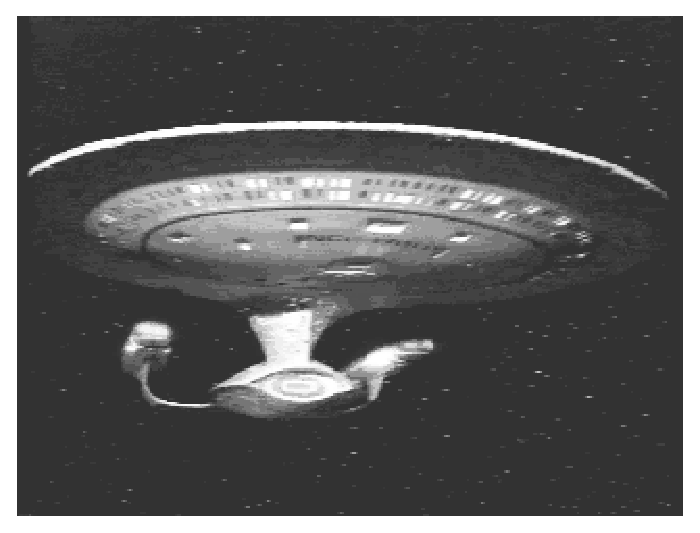
\includegraphics[height=3cm]{pics/1701.eps} &
        \includegraphics[height=3cm]{pics/ent_2e30.eps} &
        \includegraphics[height=3cm]{pics/ent_1e31.eps} \\
    \end{tabular}
\end{center}

\newpage
\subsubsection{The Andromeda Galaxy}     
This image is that of the Andromeda galaxy. A number different lenses
of varying masses were used. In all the cases the lensing object
is located in the upper left hand corner of the image [position $(0,0)$].
\begin{center}
    \begin{tabular}{cc} 
    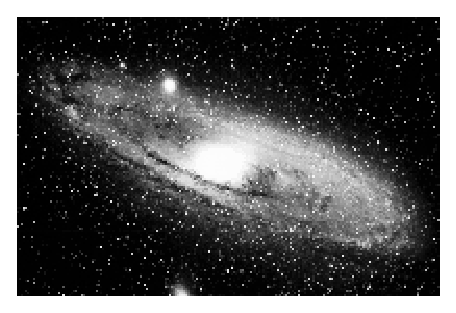
\includegraphics[height=3cm]{pics/andromeda.eps}  &
    \includegraphics[height=3cm]{pics/1e30and.eps}  \\
    $M = 0 kg$ & $M = 1 \times 10^{30}$ kg, $D = 1$ \\ 
    \includegraphics[height=3cm]{pics/1e31and.eps}  &
    \includegraphics[height=3cm]{pics/4e31and.eps} \\
    $M = 1 \times 10^{31}$ kg, $D = 1$ &  $M = 4 \times 10^{31}$ kg, $D = 1$ \\ 
    \end{tabular} 
\end{center}
As the mass of the lense is increased, the amount of distortion in the
resulting image is increased. The secondary image is also clearly visible.

\subsubsection{The Milky Way}
The image on left is looking towards the centre of the Milky Way in the
infrared. The image on the right is gravitationally lensed by a 
$M = 3 \times 10^{30}$ kg mass. The lense is located slightly left and above
from the center. This image of the Milky Way allows us to see the distortion
of the image within the Einstein radius much easier.
\begin{center}
    \begin{tabular}{cc}
        \includegraphics[height=3cm]{Pics/milky.eps} &
        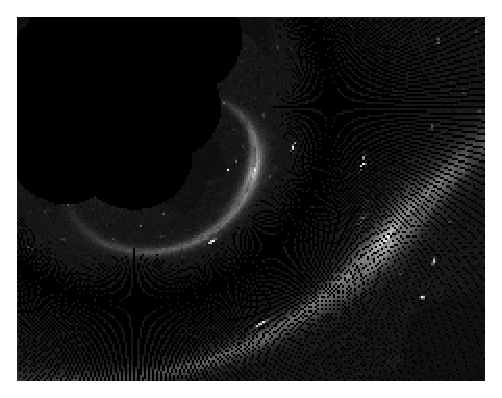
\includegraphics[height=3cm]{Pics/milky3e30.eps} \\
    \end{tabular}
\end{center}

\subsubsection{The Pleiades Star Cluster}
The image on the left is that of the Pleiades star cluster. The image
on the right is gravitationally lensed by a $M = 2 \times 10^{30}$ kg
mass.
\begin{center}
    \begin{tabular}{cc}
        \includegraphics[height=3cm]{Pics/pl.eps} &
        \includegraphics[height=3cm]{Pics/pl2e30.eps} \\
    \end{tabular}
\end{center}

\section{Caustics for the Chang-Refsdal Lens}
    \subsection{Method}
    A FORTRAN program was written (see Appendix A -- \texttt{caustics.f})
    which calculated critical curves and caustics for given
    values of $\gamma$ and $\epsilon$. As stated earlier, critical
    curves are obtained when Jacobian determinant is zero ($\det A = 0$)
    This gives:
    \begin{equation}
        \det A = 1 - \left( \gamma + \frac{\epsilon}{\bar{z}^2} \right)
                     \left( \gamma + \frac{\epsilon}{\bar{z}^2} \right) = 0
    \end{equation}.
    Using complex polar coordinates letting $z = x \cos \phi + ix \sin \phi$
    we get
    \begin{equation}
        x^4 (1 - \gamma^2) - 2 \gamma \epsilon x^2 
            (\cos^2\phi - \sin^2\phi) - 1 = 0
    \end{equation}
    The equation can be parameterised by letting:
        \[ \lambda = \cos^2\phi - \sin^2\phi \]
        \[ u = x^2 \]
    giving
    \begin{equation}
        u^2(1 - \gamma^2) - 2\gamma \epsilon \lambda u - 1 = 0.
    \end{equation}
    Solving this quadratic we obtain:
    \begin{equation}
        u = \frac{\gamma\epsilon\lambda \pm \sqrt{\gamma^2(\lambda^2 - 1) + 1}}
                 {(1 - \gamma^2)}
    \end{equation}
    For a given values of $\gamma$, $\epsilon$ and for $0 < \phi < 2\pi$
    the program calculates $u$ and then $x$. The $(x,y)$ coordinates
    for the caustic curve is then given by $(x\cos\phi, x\sin\phi)$.
    The corresponding caustics are given by:
    \begin{equation}
        y_1 = \left[ (1 + \gamma)x - \frac{\epsilon}{x} \right] 
              \sqrt{\frac{1 + \lambda}{2} } 
    \end{equation}
    \begin{equation}
       y_2 = \left[ (1 - \gamma)x - \frac{\epsilon}{x} \right] 
                     \sqrt{\frac{1 - \lambda}{2} }
    \end{equation}

    In the program a value of $\epsilon = 0.5$ was chosen. Values
    of gamma were chosen for the four representative regions in which
    caustics are found. The four regions are:
    \begin{itemize}
        \item $\gamma < -1$
        \item $-1 < \gamma < 0$
        \item $0 < \gamma < 1$
        \item $\gamma > 1$
    \end{itemize}
    The four values of $\gamma$ selected are:
    \begin{itemize}
        \item $\gamma = -1.3$ 
        \item $\gamma = -0,4$
        \item $\gamma = 0.8$
        \item $\gamma = 1.6$
    \end{itemize}

\newpage

    \subsection{Results}

    \subsubsection{$\mathbf{\gamma = -1.3}$}
    \begin{center}
        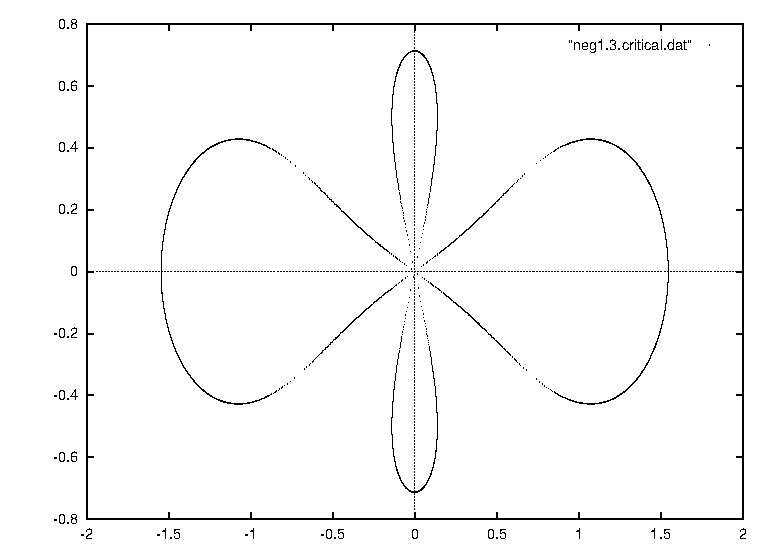
\includegraphics{images/neg1-3-critical.eps} 
        \\[1mm]
        Critical curves for $\gamma = -1.3$
    \end{center}
    \begin{center}
        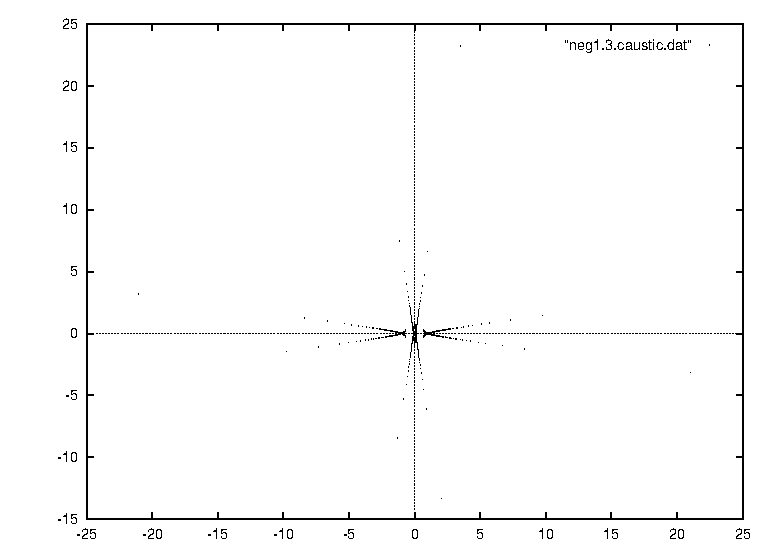
\includegraphics{images/neg1-3-caustic.eps} 
        \\[1mm]
        Caustics for $\gamma = -1.3$
    \end{center}

    \subsubsection{$\mathbf{\gamma = -0.4}$}
    \begin{center}
        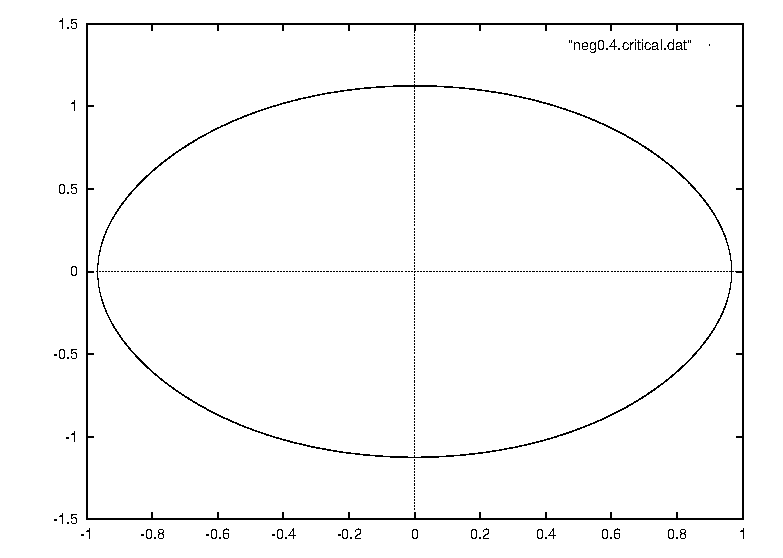
\includegraphics{images/neg0-4-critical.eps} 
        \\[1mm]
        Critical curves for $\gamma = -0.4$
    \end{center}
    \begin{center}
        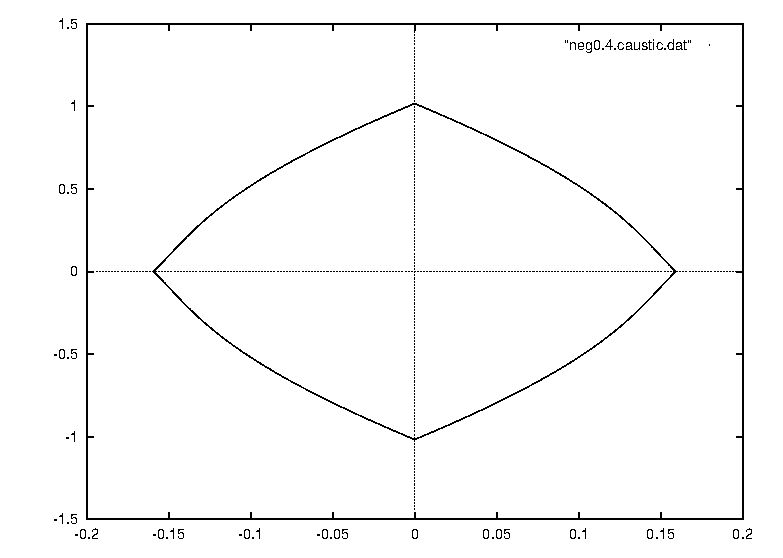
\includegraphics{images/neg0-4-caustic.eps} 
        \\[1mm]
        Caustics for $\gamma = -0.4$
    \end{center}

    \subsubsection{$\mathbf{\gamma = 0.8}$}
    \begin{center}
        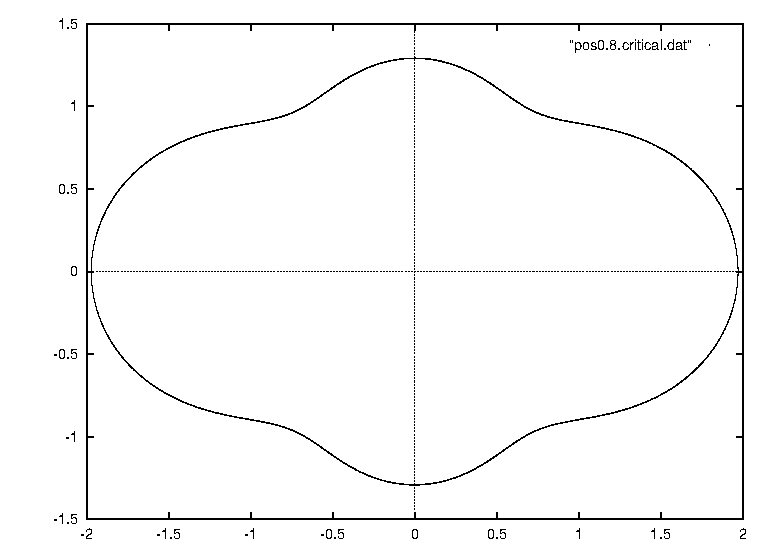
\includegraphics{images/pos0-8-critical.eps} 
        \\[1mm]
        Critical curves for $\gamma = 0.8$
    \end{center}
    \begin{center}
        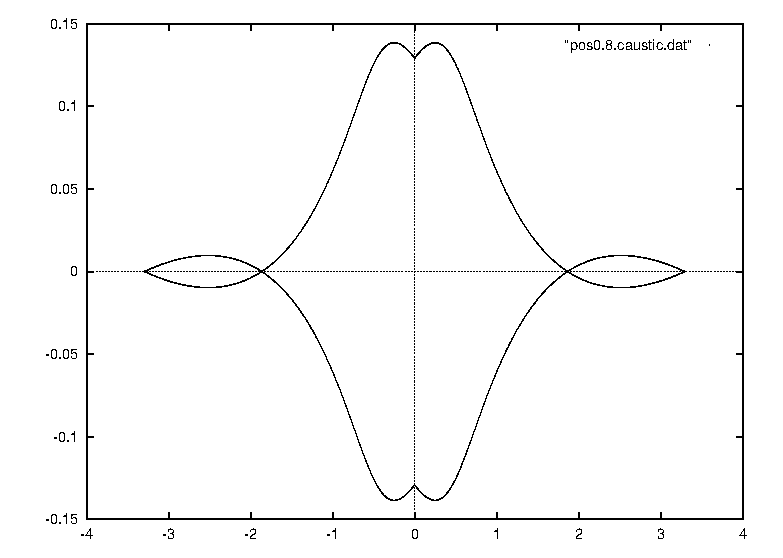
\includegraphics{images/pos0-8-caustic.eps} 
        \\[1mm]
        Caustic for $\gamma = 0.8$
    \end{center}

    \subsubsection{$\mathbf{\gamma = 1.6}$}
    \begin{center}
        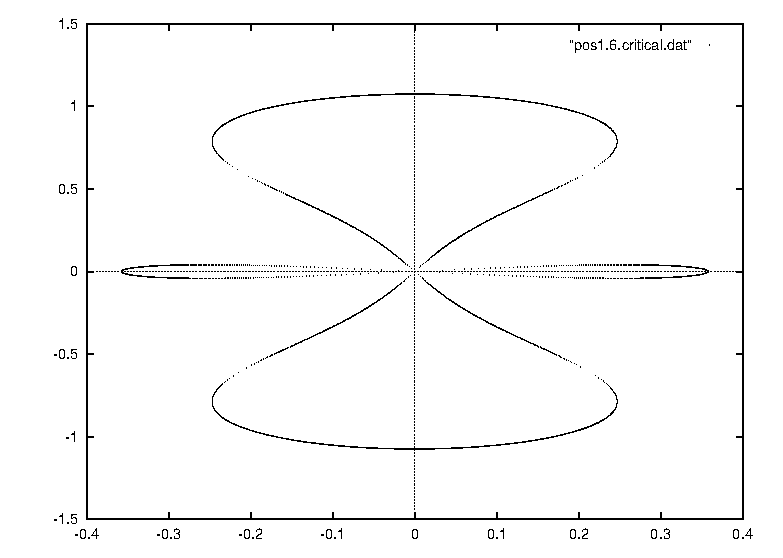
\includegraphics{images/pos1-6-critical.eps} 
        \\[1mm]
         Critical curves for $\gamma = 1.6$
    \end{center}
    \begin{center}
        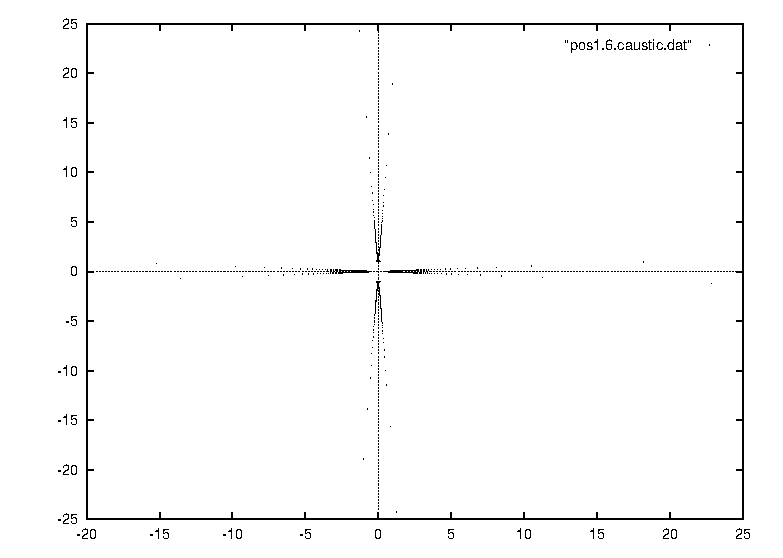
\includegraphics{images/pos1-6-caustic.eps} 
        \\[1mm]
         Caustics for $\gamma = 1.6$
    \end{center}

    \subsection{Discussion}
    As can be seen from the diagrams in the previouse section, 
    the caustic curves with values of $\gamma$ ranging between
    $-1$ and $1$ are non overlapping curves, whereas the others
    overlap in a ``petal'' pattern.

    The caustics can be used to determine light curves for background
    sources since they mark where intensity increases in the resulting
    gravitationally lensed image occur.

    \begin{center}
        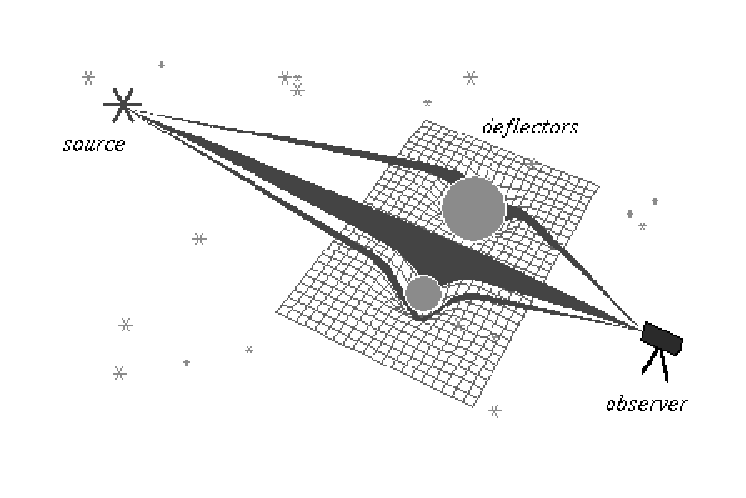
\includegraphics{images/lens_model.eps}
        \\[1mm]
        Gravitational Lensing by a Binary Star System
    \end{center}

    The use of critical lines and caustics are even more important
    when modelling graviational lenses especially when both the source
    and the lens are more complicated objects such as galaxies.
    For example, the diagram above shows the representation of 
    gravitational lensing for a distant star by a binary star system.
    As can be seen from the diagram, a simple point mass model is
    not sufficient to handle a system such as this, and hence
    more detailed models such as the Chang-Refsdal lens model
    are needed to simulate this situation so that it we can accurate
    comparisons with observations.

\appendix
% Appendix A
\newpage
\section{\texttt{caustics.f}}
\verbatimtabinput[6]{src/caustics.f}

% Appendix B
\newpage
\section{\texttt{lense.f}}
\verbatimtabinput[4]{src/lense.f}

% Appendix C
\newpage
\section{\texttt{image.c}}
\verbatimtabinput[4]{src/image.c}

\end{document}
    
